\documentclass[titlepage]{article}

\usepackage[margin=1.25in]{geometry}
\usepackage{listings}
\usepackage{enumerate}
\usepackage{amsmath}
\usepackage{color}
\usepackage{graphicx}
\usepackage{wrapfig}
%\usepackage{tikz}
\usepackage{setspace}

% \usetikzlibrary{arrows,backgrounds,calc,trees,hobby}

% \lstdefinestyle{mystyle}{                                                       
%     backgroundcolor=\color{backcolour},                                         
%     commentstyle=\color{codegreen},                                             
%     keywordstyle=\color{magenta},                                               
%     numberstyle=\tiny\color{codegray},                                          
%     stringstyle=\color{codepurple},                                             
%     basicstyle=\footnotesize,                                                   
%     breakatwhitespace=false,                                                    
%     breaklines=true,                                                            
%     captionpos=b,                                                               
%     keepspaces=true,                                                            
%     numbers=left,                                                               
%     numbersep=5pt,                                                              
%     showspaces=false,                                                           
%     showstringspaces=false,                                                     
%     showtabs=false,                                                             
%     tabsize=2                                                                   
% }

\title{Untitled}
\author{Jonathan Garcia-Mallen}
\date{??? August 2016}

\doublespacing % using package 'setspace'

\begin{document}
\lstset{language=Bash,
  numbers=left,
  stepnumber=3,    
  firstnumber=1,
  numberfirstline=true
}
\maketitle
\tableofcontents

\pagebreak

\section{Background } 
Duckietown (2.166) is a graduate class on advanced autonomy taught at MIT. It was first taught Spring 2016. It is a hands-on, project-based course focusing on self-driving vehicles and high-level autonomy. Its students work to solve the underlying problem of designing the Autonomous Robo-Taxis System for the (fictional) City of Duckietown. Its students are diverse, coming from multiple departments and with different backgrounds. 

With this diversity in mind, the first two weeks were dedicated to bringing everyone on the same page, and doling out the robo-taxis to be programmed: Duckiebots. 
    % https://docs.google.com/spreadsheets/d/1J3v3r8-toORWZah-Jqx9yEVezRbwidOiNvwpNcgwn88/edit#gid=0
A Raspberry Pi 2 
    % https://docs.google.com/spreadsheets/d/1eo5y87Vsk4pxF34WwPCUREBlYLa7RavoKfP14SQLaHU/edit#gid=0
    % inventory link
is at the center of these machines. To program them, students learn to log in remotely from their laptops to the robot's Pi and launch programs the same way, or by sending a command directly from their laptops without logging into their robot. The students have no way of running a program on their duckiebots without using their laptops.

Picture this scenario. A grad student is testing a new autonomy on his laptop. His research advisor happens to walk by on her way to a meeting and asks him ``how's your duckiebot doing?'' The student hurries excitedly to power on his robot taxi (named batmobile), waits for it to connect to the network, and rushes the following incantation into his laptop's terminal:
% change 'dat-grad-student' to 'you'?

% ah thank ye Jesus for waking me up at 0614 here in NH,
% letting me exercises, bathe go to morning prayer, pray a little more, and then making time for me to write her. Te lo agradezco, sinceramente. 
\begin{verbatim}
  dat-grad-student@duckietop4:~$ ssh batmobile
  ssh: Could not resolve hostname batmobile.local: Name or service not known
  dat-grad-student@duckietop4:~$ ping batmobile.local
  ping: unknown host batmobile.local
  dat-grad-student@duckietop4:~$ ping batmobile.local
  PING cepillo.local (10.42.0.62) 56(84) bytes of data.
  64 bytes from 10.42.0.62: icmp_seq=1 ttl=64 time=1.02 ms
  64 bytes from 10.42.0.62: icmp_seq=2 ttl=64 time=0.971 ms
  ^C
  --- batmoble.local ping statistics ---
  2 packets transmitted, 2 received, 0% packet loss, time 1001ms
  rtt min/avg/max/mdev = 0.971/1.000/1.029/0.029 ms
  dat-grad-student@duckietop4:~$ ^C
  dat-grad-student@duckietop4:~$ ssh batmobile
  ubuntu@batmobile:~$ roslaunch duckietown dat-grad-students-demo.launch  veh:=batmobile
 \end{verbatim}

First, \texttt{ssh batmobile} is run to log into the duckiebot named batmobile. Failing that, the student \texttt{ping}s his robot to see if it is on the network. On the second ping attempt, batmobile has completed enough of its bootup sequence to respond to pings. The student \texttt{ssh}'s into batmobile and launches his demo. But by this time, his advisor has already walked on to her meeting. 

This is clearly a worst-case scenario. It is not the only scenario.
% rephrase previous sentence. Don't repeat 'scenario'.
A well-planned demo for a barely-technical audience would demand questions such as "Why do you need a laptop, if this is an autonomous vehicle?" or "Is the code running on the robot, or your computer?" A laptop and the corresponding WiFi network necessary are other potential points of failure. Trying to demonstrate your robot in a lab with twenty other duckiebots clogging the same 2.4GHz channel can lead to frustrations best kept outside of the scope of 2.166. A laptop should not be necessary in order to begin an autonomous routine on the duckiebot. This 6.UAP project remedies this. 
\section{Requirements and Design Goals}
The purpose of this project is to create a quick and easy means to start any ROS program on the duckiebot. There is a clear primary requirement: this system must let the user (researcher or student) start a program of their choosing on the duckiebot without using a computer offboard the robot. Its Raspberry Pi has two inputs that may be considered: a Raspberry Pi Cam 2, and a Logitech Gamepad F710 joystick controller. The computer itself runs Ubuntu 14.04.

Three goals guided the fulfillment of this requirement. The system must be reliable. It cannot fail when the user is in front of an audience. It must be easy to use and require as little interaction as is possible. Users shouldn't have a hard time interfacing with it, or have to push more buttons than when they type in roslaunch.
% awkward wording
Lastly, this implementation must be future-proof. The duckietown software will migrate to  different versions of ROS and Ubuntu. The utilities produced by this project must be usable even as ROS and Ubuntu change. 
\section{Existing technologies used} 
% code/shell should definitely be moved from this section to the next
We must start a program at an unexpected time. Using input directly to the Raspberry Pi. We use its joystick. Input from the joystick must always be monitored. This monitor, this daemon, must start up on the duckiebot by itself. 

To interface with the joystick, we included this python module from github. 
The initialization system initializes every process that runs on Ubuntu, directly or indirectly. But both used by Ubuntu 14.04 have been marked for death.
Supervisord is a python package that can also initialize and manage processes. It is actively developed by several dozen contributors on github.
We explain these three subsystems here. 
\subsection{js\_linux.py}
Nearly everything is a file in a UNIX operating system such as Ubuntu. This includes inputs from the joystick. When a button is pressed or a joystick is tilted, the events are written to a file \texttt{/dev/input/js0}. We use python to directly open and read this file:

\begin{lstlisting}
  # Open the joystick device.
  fn = '/dev/input/js0' 
  print('Opening %s...' % fn)
  jsdev = open(fn, 'rb')
\end{lstlisting}

This snippet is from js\_linux.py [1]. This script reads and also parses this. When run, it prints to the terminal what buttons are being pressed and how much a joystick's axis is being tilted. We modify js\_linux.py in order to import it as a module. 

This script is based on the more standard C api for reading events written by the joystick device. The python script was chosen over the C api so that more people would be able to understand how these modules work, and modify them if they see it necessary. More MIT students are familiar with python than with C, especially when one considers undergraduate students.
\subsection{System V}
We want Ubuntu  to start a processes that listens to joystick commands, and we want it to start it when Ubuntu boots up. This background listening program is also called a daemon. 

Starting up Ubuntu is a process. The computer is powered on, the master boot record is read from disk, it then calls the boot loader (grub), and grub calls Linux. Linux calls the process that initializes (directly or indirectly) all other processes in Ubuntu. 
In Ubuntu 14.04, there are two such initialization processes: upstart and System V (sysv). % cite something
The directories /etc/init and /etc/init.d correspond to either system, respectively. These directories contain scripts to be started by the init system. Each system has its own syntax for their init scripts. 

Both init systems are in the process of being depreciated. Their replacement, systemd, is not readily available for Ubuntu 14.04. 

We use sysv to indirectly start our joystick daemon. It has much greater support than upstart. To use sysv for stating a program automatically when Ubuntu boots, we write a sysv init script in /etc/init.d.

This init script does not start the listening program. It is used to start supervisord. 
\subsection{supervisord}
Supervisor (supervisord) is a process control system [3]. It facilitates monitor and control of processes, and it is meant to start at boot time. It does not replace init, but is called by our init script into action. Upstart and sysv are being depreciated, and supervisord is much easier to interact with than an init script. It is configured via the \texttt{/etc/supervisor/supervisor.conf} configuration file.

We use supervisord version 3 as it allows us to run processes as a specific user. How this would be done in init scripts has not been found. This version had to be installed via pip, as the Ubuntu 14.04 package repositories only contain older versions. This feature is crucial, and is not available in older versions. 

Installing via pip rather than apt-get required us to make an init script for it. This is not required in newer versions of Ubuntu. Unlike a System V init script, Duckietown can continue using Supervisord after transitioning to a newer version of Ubuntu, when the time comes to do so. And as it is developed by dozens [4] of developers, supervisord is a dependency Duckietown can depend on.
\section{Implementation}
% the subsection will be the individual files / indivisible components. 

Here we explain the code written specifically for this project. The software fits in one of two tasks. The joystick daemon launches commands upon button press. The startup scripts and configuration files ensure the daemon is running in the background after the duckiebot boots up. 

\begin{wrapfigure}{r}{0.5 \textwidth}
  \centering
  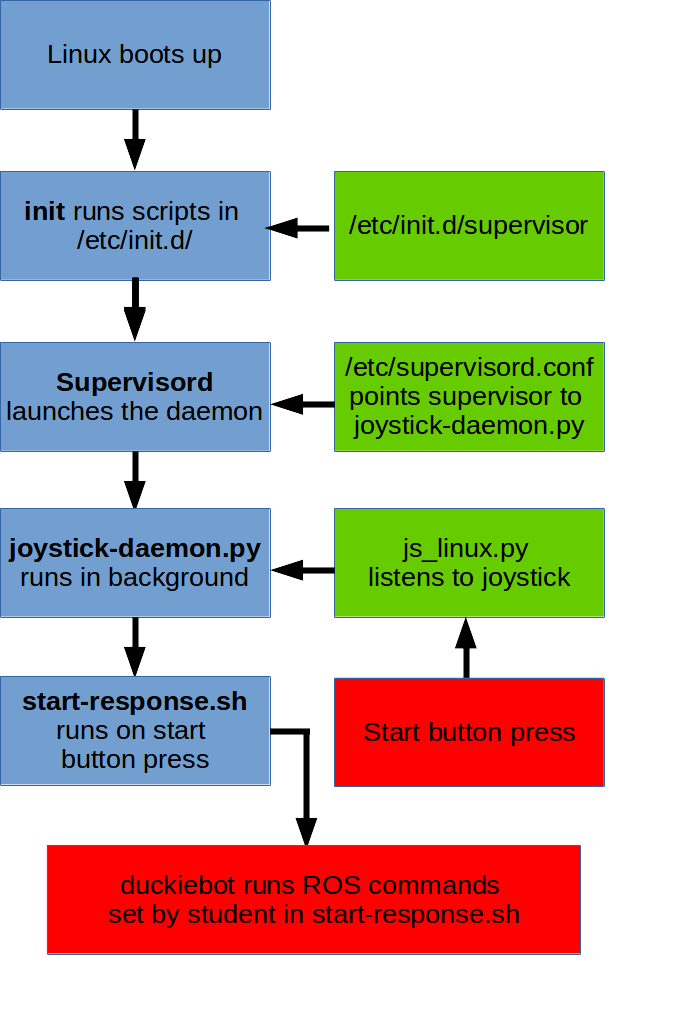
\includegraphics[scale=0.422]{system_diagram.png}
\end{wrapfigure}

The joystick daemon itself and its interface to users was demonstrated to work consistently in April 2016.
It consists of three parts. The aforementioned js\_linux.py is used as a module by joystick-daemon.py to parse joystick input. joystick-daemon.py then calls then sits in the background listening for inputs. The last part is shell scripts corresponding to joystick buttons. Here, users write the commands they want to run on a certain button press. 

The second part of this project revolved around starting the joystick daemon every time the Raspberry Pi was powered on. While typically a simple task, the problem of starting the joystick daemon quickly overshadowed the daemon itself. The usual method, rc.local, was unreliable. An init.d script was also troublesome, though a different one consistently started supervisord. This last module worked for us in August 2016.

\subsection{Joystick Daemon}
The joystick daemon consists of three parts: js\_linux.py, joystick-daemon.py, and shell scripts corresponding to the buttons on the joystick.  
\subsubsection{joystick-daemon.py}
joystick-daemon.py sits in the background running the below abridged infinite loop. It is based off of an example from js\_linux.py. We have modified js\_linux.py by adding \texttt{if \_\_name\_\_ == '\_\_main\_\_':} before its own loop. This way, joystick-daemon.py can import js\_linux.py as a module. Here is our main event loop from joystick-daemon.py:
\begin{lstlisting}
    while True:
        event_buffer = jsdev.read(8)  # jsdev is defined i js_linux.py
        if event_buffer:
            time, value, type, number = struct.unpack('IhBB', event_buffer)

        # If the event type is a button press 
        if type & 0x01:
            button = button_map[number]  #b button_ma
            if button:
                button_states[button] = value
                if value and button == 'start':
                    subprocess.call([start-response.sh'])
\end{lstlisting}
Each iteration, in lines two and three, we check to see if an event has been written to /dev/input/js0. If the event is a button press, it checks which button was pressed and calls the shell script corresponding to this buffer. For example, if the start button is pressed, joystick-daemon.py will call start-response.sh.

jsdev and button\_map are defined in js\_linux.py. jsdev is a file object pointing to /dev/input/js0. button\_map is a python list mapping the button's id on the jostick with the button's english name. In line eleven, that button is the start button. 
\subsubsection{start-response.sh}
This shell script is called by joystick-daemon.py whenever the start button is pressed. In order to run a ROS program, one usually performs the following invocation while logged into the duckiebot:

\begin{lstlisting}
  source /home/ubuntu/duckietown/environment.sh;
  source /home/ubuntu/duckietown/set_ros_master.sh;
  roslaunch duckietown new-autonomy.launch veh:=batmobile;
\end{lstlisting}

The first two lines set up ROS so that it may be used. The third  launches the desired program; here, our grad student's new-autonomy.launch is launched on the vehicle named batmobile.

\subsection{Launching the Daemon} 
% \subsubsection{(runlevels, if need more padding)}
We want to launch our daemon every time the vehicle powers on. A separate startup script must call it. This startup script must run joystick-daemon.py as the user 'ubuntu' without fail whenever the robot is powered. 

The entire duckietown software is kept in /home/ubuntu/duckietown for every duckiebot. 'ubuntu' is the username for all Raspberry Pi's on each duckiebot. Since the software is located and set up for the user ubuntu, it must be run as ubuntu. Numerous attempts were made to run an example joystick.launch progam as the root user, as most start scripts are run. We did not succeed in this.

\subsubsection{rc.local}
The easiest method of running a program on startup in ubuntu is by modifying /etc/rc.local. By default, this script does nothing. It is executed as the root user at certain stages of the startup process. We added a line similar to this the file:
\begin{lstlisting}
  su ubuntu -c "python /home/ubuntu/.duckietown/joystick-daemon/joystick-daemon.py >> /dev/null" &                                                            
\end{lstlisting}

the \texttt{su} command lets one run commands as a different user. Here, root uses su to run python as user ubuntu. Unfort
This method successfully called the startup script at about 50\% of all boot sequences. 
We were not able to find out why it failed half the time, so we investigated other methods.

\subsubsection{init.d}
We first tried to run joystick-daemon.py directly from a sysv init script. Seeing little promise there, we then modified an init script for supervisord from Ubuntu's repositories. 

Creating a sysv init script is the standard method of starting a program upon system boot. 
It is a single file in /etc/init.d that adheres a certain format. 
After sysv is made aware of the new script, the scripts corresponding daemon is run after the specified st
We wrote /etc/init.d/duckietown\_joystickd as such a script, but its several iterations had unique issues. 
The initial complexity of sysv was the first, followed by difficulties in running the daemon as user ubuntu.
Ideally, this project would have used a sysv init script to call joystick-daemon.py directly. 

Instead, we use supervisord version 3.3.1 to run joystick-daemon.py as user ubuntu. We used pip to install version 3.3.1 from the Python Package Index, but it did not configure an init script for itself. Ubuntu 14.04's package repositories have one for version 3.0b2-1, but this version does not have the feature we need. We modified 3.0b2-1's init script to work with 3.3.1. 

The modifications were few. Ubuntu provides a 160 line long example init script: /etc/init.d/skeleton. Four lines are relevant for starting Supervisord:
\begin{lstlisting}
PATH=/usr/local/sbin:/usr/local/bin:/sbin:/bin:/usr/sbin:/usr/bin
  DAEMON=/usr/local/bin/supervisord
  NAME=supervisord
  DESC=supervisor
\end{lstlisting}

With this sysv init script, Supervisord consistently ran upon system startup. 
\subsubsection{supervisord}
Just a sledgehammer can successfully crack a walnut, supervisord successfully runs joystick-daemon.py every time the duckiebot is booted. 
It is started when its init script, /etc/init.d/supervisor, is called by the init system. 
Supervisord in turn calls joystick-daemon.py via a program block within its configuration file /etc/supervisor/supervisor.conf:

\begin{lstlisting}
  [program:joystickd]
  command=/usr/bin/python                                          \
      /home/ubuntu/.duckietown/joystick-daemon/joystick-daemon.py  \
      >> /dev/null
  umask=022
  user=ubuntu
\end{lstlisting}

Thus, it succeeds in initializing the python listening script. 

% \section{Example}
% Here we briefly walk through an example. 
% dat grad wants to run my-super-duper-autonomy.launch whenever he presses the start button. 

\section{Conclusions and Future work}
The base goal of a reliable, future-proof interface was tested by cutting and reestablishing power to the duckiebot ten times and pressing the start button on the joystick to launch the joystick demo. Running the joystick demo lets the user drive the duckiebot using the joystick. Each time, pressing the start button and waiting about fifteen seconds let the user drive the duckiebot with the joystick. The program started 10/10 times. 

It should not have taken this long to do this project. Had rc.local been reliable, this likely would have been finished in may. Unfortunately, no. 

we use ROS, arguably the most popular robotics middleware around. That didn't matter much at all for this project. This entire system could be used for a system running on MOOS, used by LAMSS, or LCM, used by the Robot Locomotion group. So long as a joystick is being used as input, the only file that would change would be start-response.sh.

\textbf{Future Work:} \\
consider using sysv init. I did not consider it at all. However, supervisord is a very large dependency; an oversized cludgeon for the little nail of a problem we have. Considerations: What are the differences between 14.04 init and 16.04 init? 

The dependency of supervisord must be removed. The latest this should happen is when Duckietown switches to Ubuntu 16.04. 

It should be more user friendly.  
\subsection{Acknowledgements}
\begin{itemize}
\item John Leonard, CEO(???) of Duckietown Engineering Co., for generously advising this and many others of my works
\item Liam Paull, COO of Duckietown Engineering Co., for advising me directly and patiently
\item Alex Chernovsky, of SIPB, for recommending supervisord
\item Anders, of pika, for giving me advice, though I forgot that advice
\item that person from office of EECS undergrads, for helping me get an incomplete when jleonard was busy
\item Kelly Shen, for planning advice, writing examples, and prayers. 
\end{itemize}

\subsection{References}
\begin{enumerate}[(1)]
\item rdb had a nice gist on github.com https://gist.github.com/rdb/8864666
\item original C api for the joystick https://www.kernel.org/doc/Documentation/input/joystick-api.txt
\item supervisord exists at http://supervisord.org/
\item https://github.com/Supervisor/supervisor/graphs/contributors <-- supervisord has devs.
\item we used pip! https://pypi.python.org/pypi/supervisor/3.3.1
\end{enumerate}

\end{document}



%  LocalWords:  systemd sysv py Supervisord supervisord init linux js
%  LocalWords:  rc startup dev duckiebot ubuntu username
